\documentclass[conference]{IEEEtran}
\IEEEoverridecommandlockouts
% The preceding line is only needed to identify funding in the first footnote. If that is unneeded, please comment it out.
\usepackage{cite}
\usepackage{amsmath,amssymb,amsfonts}
\usepackage{algorithmic}
\usepackage{graphicx}
\usepackage{textcomp}
\usepackage{xcolor}
\def\BibTeX{{\rm B\kern-.05em{\sc i\kern-.025em b}\kern-.08em
    T\kern-.1667em\lower.7ex\hbox{E}\kern-.125emX}}
\begin{document}

\title{Analysis of Crimes against Male-Female Employment and Tourism in SriLanka\\
{\footnotesize \textsuperscript{*}Note: Sub-titles are not captured in Xplore and
should not be used}
\thanks{Identify applicable funding agency here. If none, delete this.}
}

\author{\IEEEauthorblockN{1\textsuperscript{st} Waruna Priyankara}
\IEEEauthorblockA{\textit{dept. Computer Science and Engineering} \\
\textit{University of Moratuwa}\\
Moratuwa, SriLanka \\
199371p@uom.lk}
\and
\IEEEauthorblockN{2\textsuperscript{nd} Prageeth Anjula}
\IEEEauthorblockA{\textit{dept. Computer Science and Engineering} \\
\textit{University of Moratuwa}\\
Moratuwa, SriLanka \\
199304p@uom.lk}
\and
\IEEEauthorblockN{3\textsuperscript{rd} Pumudinee Kumarasiri}
\IEEEauthorblockA{\textit{dept. Computer Science and Engineering} \\
\textit{University of Moratuwa}\\
Moratuwa, SriLanka \\
email address}
\and
\IEEEauthorblockN{4\textsuperscript{th} Hesitha Wijayasinghe}
\IEEEauthorblockA{\textit{dept. Computer Science and Engineering} \\
\textit{University of Moratuwa}\\
Moratuwa, SriLanka \\
199372u@uom.lk}
}

\maketitle

\begin{abstract}
Increasing of crime related activities is a big problem for any country.
The third world country like SriLanka suffers from crimes a lot. This affects 
to the growth of economy of the country as well as increment of social problems.
Theoretical and application-oriented approaches which provide insights into why and where crimes take place are more valuable for decision and policy makers.
Geographic information systems and graphical analysis are proving to be essential for studying criminal activities.This paper explores how criminal data relate with male-female employment and tourism industry in SriLanka.
\end{abstract}

\begin{IEEEkeywords}
data science, hypothesis, analysis, statistics
\end{IEEEkeywords}

\section{Introduction}
Number of data sets are freely available at Open Data Portal \cite{b2} of SriLanka which is an initiative of SriLanka government to facilitate researches, policy makers and decision makers to come up with ideal solutions for prevailing problems. Crime is a serious problem in SriLanka. Crime related news are published in newspapers each and every day. Authors have chosen data mentioned in Table ``Tab.~\ref{tab1}'' to analyze about criminal activities and their relation between tourism and employment.
Before giving solutions for criminal activities the true reasons behind crimes should be understood. Authors want to see whether there are correlation of crime data with employment and tourism. These data has been recorded as district base. Before analyzing three sets were integrated together. The primary contributions of this paper are:
\begin{itemize}
\item Analyze crime data and male-female employment data for correlation
\item Analyze crime data and tourism data for correlation
\item Use scientific methods in data science for processing, analyzing and visualization
\end{itemize}

\begin{table}[htbp]
\caption{Data set Details}
\begin{center}
\begin{tabular}{|p{3cm}|p{6cm}|}
\hline
\textbf{Data Set}& \textbf{Link}\\[14pt]
\hline
Crime data 2010-2012 & http://www.data.gov.lk/dataset/crime-data-2010-2012 \\[5pt]
Employment by Industrial Sector 2012& http://www.data.gov.lk/dataset/employees-industrial-sector-2012\\[5pt]
Accommodation information for tourists& http://www.data.gov.lk/dataset/accommodation-information-tourists\\[5pt]
\hline
\end{tabular}
\label{tab1}
\end{center}
\end{table}

\section{Data and Methodology}

\subsection{Data}
Data set and reference to open data portal is mentioned in Table ``Tab.~\ref{tab1}''. Data set dimensions are mentioned below
\begin{itemize}
    \item Crime Data set size =  (25, 23)
    \item Employment Data set size =  (25, 13)
    \item Tourism Data set size =  (2130, 7)
    \item Integrated dataframe shape =  (25, 36)
\end{itemize}
Extortion, abduction, rape ``Fig.~\ref{fig_geo}'' crime data distribution throughout the country were plotted.How male-female employment vary across district and room count(``Fig.~\ref{fig_rooms}'') distribution were also plotted. We can observe that the employed female population is higher than employed male population in most district. At the same time hotel room count is also higher in those districts. 
\begin{figure*}[htbp]
  \centering
    \subfloat{{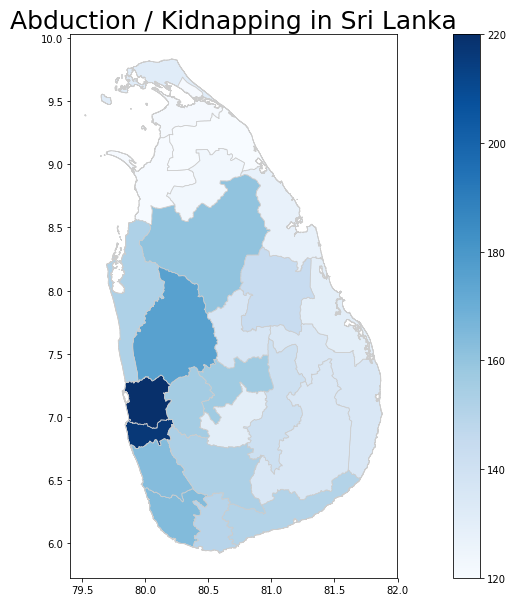
\includegraphics[width=6cm]{crime_abduction.PNG} }}
    \qquad
    \subfloat{{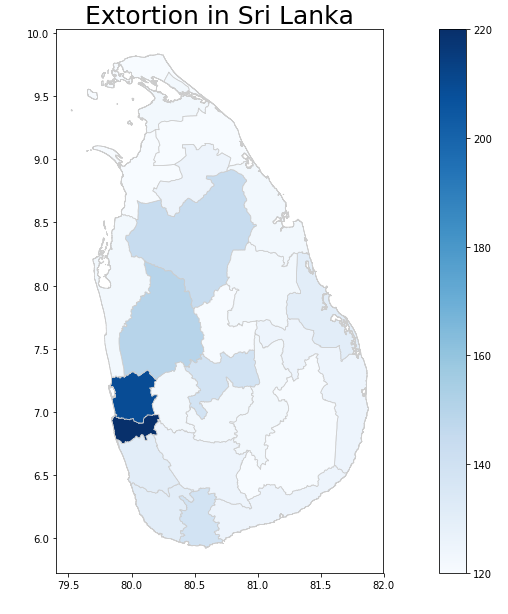
\includegraphics[width=6cm]{crime_extortion.PNG} }}
     \qquad
    \subfloat{{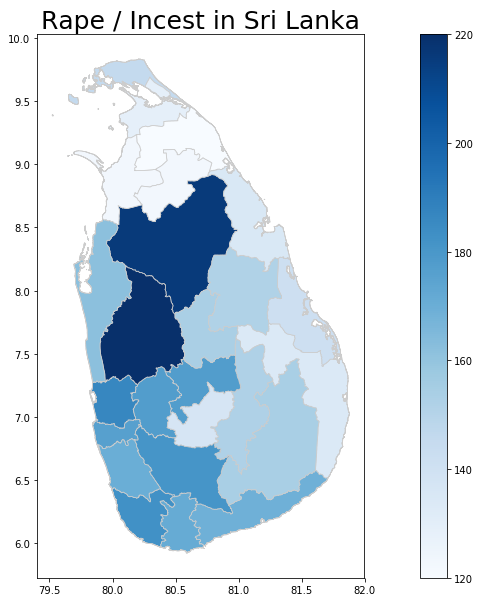
\includegraphics[width=6cm]{crime_rape.PNG} }}
    \caption{Geo maps for crime}
  \label{fig_geo}
\end{figure*}

\begin{figure*}[htbp]
    \centering{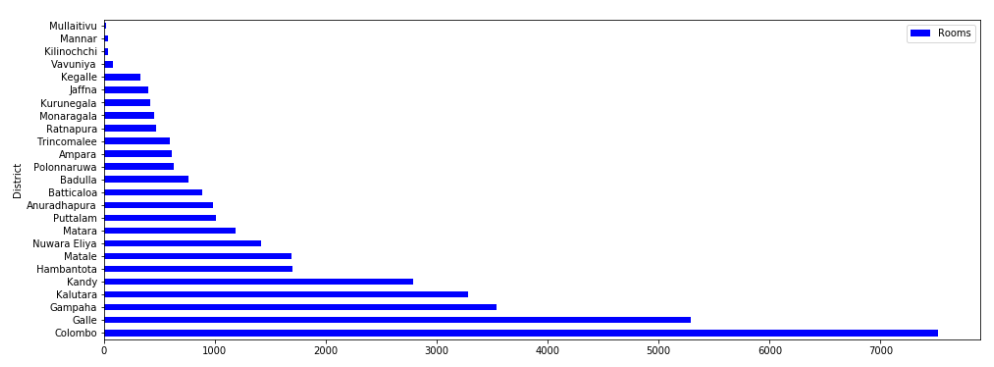
\includegraphics[width=\textwidth,height=8cm]{rooms.PNG} }
    \caption{Room counts}
    \label{fig_rooms}
\end{figure*}

\subsection{Methodology}
We used 'pandas' python framework to load and analyze data. Initially data was loaded to separate data frames. Integrating them to one data frame was a challenge. District is common factor in every data set. Crime data set and employment data set were sorted on District. From tourism data only room count was taken per district. Then data frames were merged together to get the final integrated data frame. 
Room count correlation(Pearson) was calculated and heat map was created for correlation coefficient which is greater than 0.75. ``Fig.~\ref{fig1}'' shows that room count shows a high correlation with almost all crime data. Robbery, Abduction/kidnapping, Offence under Dangerous drugs, Home break and theft are highly correlated. ``Fig.~\ref{scatter}'' shows scatter plots of each crime and tourism room count.Colombo, Galle, Gampaha, Kandy, Kalutara is booming with tourism, so as crimes. All these has more than 2000 tourist rooms, which is popular for tourists.
A correlation between female employment in industry sector and crime data is also detected. Especially abduction/kidnapping, Home break and theft, Hurt by knife are highly correlated. 

\begin{figure*}[htbp]
\centerline{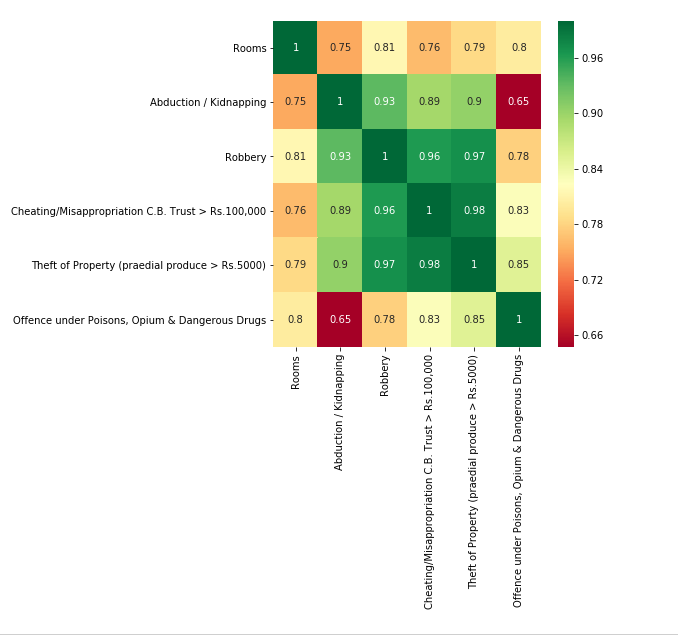
\includegraphics[width=\textwidth,height=12cm]{fig1.PNG}}
\caption{Heat map of room count with crimes.}
\label{fig1}
\end{figure*}

\begin{figure*}[htbp]
\centerline{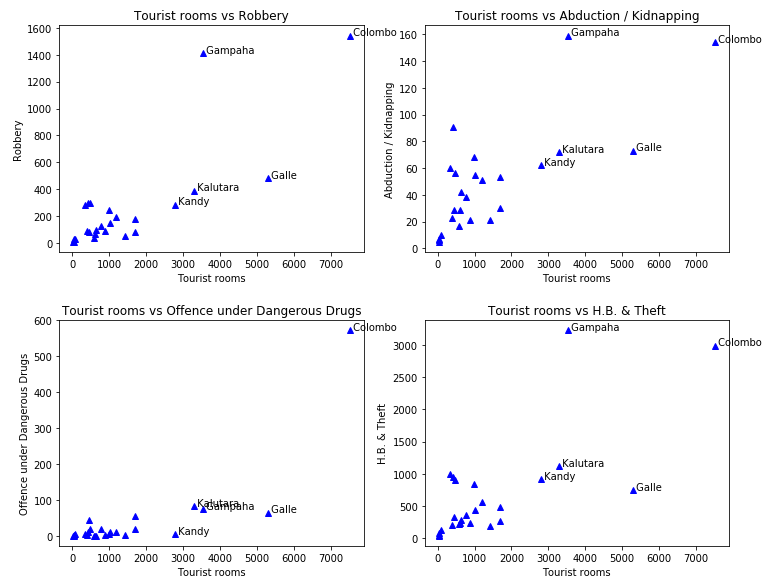
\includegraphics[width=\textwidth,height=12cm]{scatter1.PNG}}
\caption{Scatter plots for crime vs tourism rooms.}
\label{scatter}
\end{figure*}

\section{Results}
After analyzing relationship between crime and tourism/female employment were observed.``Fig.~\ref{scatter}'' and ``Fig.~\ref{scatter2}'' show how each variable relates crime data.




\section{Conclusion}
There is no doubt that tourism is often a driving force for a given region, city or country. Tourism attractiveness is a blessing for an area, a town or site. Tourism represents a main portion of GDB in SriLanka too. As our results shown there is a big relationship with tourism and crime. Criminal activities are higher in tourism areas. These activities may be on tourists or locals. Eventually this will result in reducing tourist attraction in those areas. This is directly affected to the economy as well. This will also affect to the quality of citizens’ lives. Therefore security is a very important factor when deciding a tourism destination. Most of the time most crimes committed against tourists are not reported because
\begin{itemize}
    \item Most tourists are not immediately aware that they have become victims of crime.
    \item Sometimes the victim does not know what to do after s/he has been attacked and where to go and whom to report it to. Thus it is easier to forget about the matter.
    \item Sometimes the victims are often convinced that they will not regain the stolen items so it is useless for them to report the incident.
\end{itemize}
Because of those reasons the actual data should be further increased. There is no doubt that tourism and crime are common phenomena. Countries like SriLanka tourism is the easiest route to rapid development. Therefore government should concern about this phenomena and take necessary actions to resolve these issues.  

\begin{figure*}[htbp]
  \centering
    \subfloat{{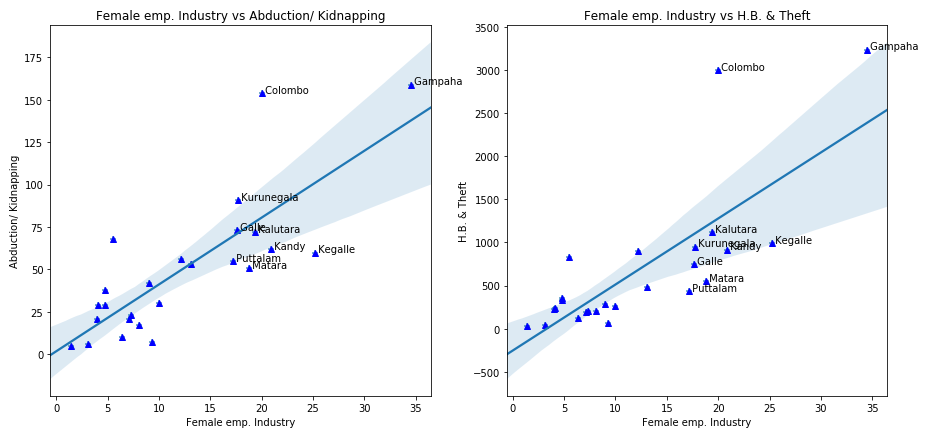
\includegraphics[width=\textwidth,height=8cm]{scatter2.PNG} }}
    \qquad
    \subfloat{{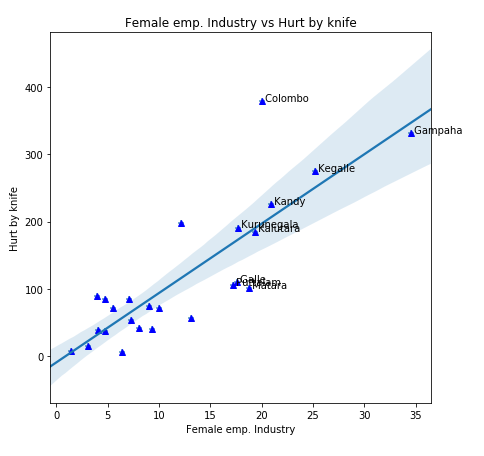
\includegraphics[width=10cm]{scatter3.PNG} }}
    \caption{scatter plot for crime vs female employment}
  \label{scatter2}
\end{figure*}

\begin{thebibliography}{00}
\bibitem{b1} Agnieszka Lisowska, ``crime in tourism destinations: research review,'' Agnieszka Lisowska University of Wroclaw, Institute of Geography and Regional Development,.
\bibitem{b2} open data portal, "http://www.data.gov.lk/".
\bibitem{b3} Discover the beauti of Latex , ``https://www.latex-tutorial.com/'' .
\end{thebibliography}

\end{document}
